The results in 1D are very promising, but the real open challenges are situated in 2 (or higher) dimensions. Therefore, it is an interesting and relevant question whether the results generalise to 2D. These results are twofold. On the one hand, a similar measure as in 1D is calculated to measure how good a method works on a specific 2D grid. Here, we will need to settle for what can be computed. As a second measure, and from physical point of view the most interesting one, some phase transitions of the 2D transveral Ising model are determined, and compared against values in literature.

\subsection{Norm}

Once again, a suitable norm has to be derived. The situation is more difficult than in 1D, because contracting a PEPO tensor network has a much larger computational complexity than in 1D. Ideally, the norm would be calculated on a nxn cyclical grid (2D grid on a torus). Here n has to be at least 1 larger than the largest explicitly constructed chain.

In practice, this is not achievable in reasonable amount of time. The limitations are twofold: the maximum number of sites to calclate the matrix exponential is still around 14, and the contraction of the tensor network on a torus is limited to 3 by 3. This not capture the long chains.

The limitations on the PEPO contraction can be somewhat relaxed by not computing the full network, but computing the reduced density matrix. Here, most of the sites have their physical indices traced out, except for one site.

The final error measures are defined by:
\begin{equation}\label{res2d:err_Def}
    \rho^1_{i,j} =\vcenter{ \hbox{ \pepob{8}{8}{{
                        "-","-", "-","-","-","-","-",
                        "",  "", "","","","","",
                        "",  "", "","","","","",
                        "",  "", "","","","","",
                        "",  "", "","","","","",
                        "",  "", "","","","","",
                        "",  "", "","","","","",
                        "-", "-", "-","-","-","-","",}}{{
                        "-","-", "-","-","-","-","-",
                        "","", "","","","","",
                        "","", "","","","","",
                        "","", "","","","","",
                        "","", "","","","","",
                        "","", "","","","","",
                        "","", "","","","","",
                        "-","-", "-","-","-","-","",}}{{
                        1,13,1,1,1,1,1,1,
                        1,0,1,1,1,1,1,1,
                        1,0,1,1,1,1,1,1,
                        1,0,1,1,1,1,1,1,
                        1,0,1,1,1,1,1,1,
                        1,0,0,0,1,1,1,1,
                        13,12,0,0,0,0,0,13,
                        1,13,1,1,1,1,1,1,
                    }} }}
\end{equation}
and
\begin{equation}\label{res2d:err_Def}
    \rho^2_{i,j} =\vcenter{ \hbox{ \pepob{8}{8}{{
                        "-","-", "-","-","-","-","-",
                        "",  "", "","","","","",
                        "",  "", "","","","","",
                        "",  "", "","","","","",
                        "",  "", "","","","","",
                        "",  "", "","","","","",
                        "",  "", "","","","","",
                        "-", "-", "-","-","-","-","",}}{{
                        "-","-", "-","-","-","-","-",
                        "","", "","","","","",
                        "","", "","","","","",
                        "","", "","","","","",
                        "","", "","","","","",
                        "","", "","","","","",
                        "","", "","","","","",
                        "-","-", "-","-","-","-","",}}{{
                        1,1,1,1,1,1,1,1,
                        1,1,1,1,1,1,1,1,
                        1,1,1,1,1,1,1,1,
                        1,1,1,1,1,1,1,1,
                        1,1,1,0,0,1,1,1,
                        1,0,0,12,0,0,0,1,
                        1,0,0,0,0,0,0,1,
                        1,1,1,1,1,1,1,1,
                    }} }}
\end{equation}
For the first one, all the blocks in the expansion are present in, and it is cyclical in both x and y. The second reduced density matrix is not cyclic, but includes more loop type contributions. Both relative errors will be used, defined by :
\begin{equation}\label{eq:2d_norms}
    \epsilon^{\alpha} = \frac{  {  \left \|  \rho^{\alpha}_{exact,  i,j}- \rho^{\alpha}_{ i,j}  \right \|} _{2}  }{ {  \left\|  \rho^{\alpha}_{exact,  i,j} \right \|}_2} \quad \alpha \in [1,2]
\end{equation}
For the given error measures, series expansion up till order 5 can be tested. The second norm takes the most time to compute, due to the larger complexity of contracting the tensor network.

\subsection{Models}

\subsubsection{Ising}

For this test, the cluster expansion is of order 5, and the transversal field is of magnitude $g=2.5$. The results can be seen in \cref{fig:res2d:n1:tising}.

There are 3 different constructions: without loops, only plaquette term (\cref{tikzfig:plaquetter}) and with loop extensions from one corner (\cref{eq:s_loop_ext}). This is tested for both norms (see \cref{eq:2d_norms}).

The plaquette term (\cref{tikzfig:plaquetter}) is mainly important at low $\beta$. It also improves the error at $\beta \approx 1$ considarably. The extensions improve the results slightly, but at large cost in bond dimension.

Both norms show the same trend, with norm $\epsilon^2$ being somewhat more strict. Of course, the real norm for an infinite lattice is even more restrictive than both norms calculated.

\begin{figure}
    \center
    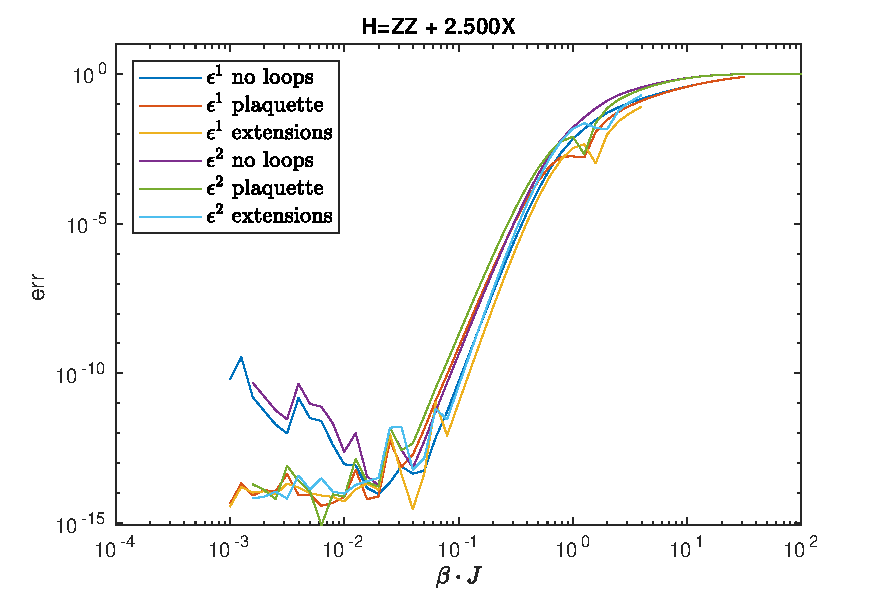
\includegraphics[width=\textwidth]{Figuren/benchmarking/2D_Err01_t_sing.pdf}
    \caption{The errors $\epsilon^i$ for 2D transveral field Ising model. }
    \label{fig:res2d:n1:tising}
\end{figure}
\todo{fix caption}

\subsubsection{Heisenberg}

The results for the harder to simulate Heiseberg model are shown in \cref{fig:res2d:n1:heis}. The conclusion is once again that the error $\epsilon^2 > \epsilon^1$ most of the time. The loops are absolutely a big improvement for  the results at low $\beta$. The loop extension also help to lower the error considerably.

\begin{figure}
    \center
    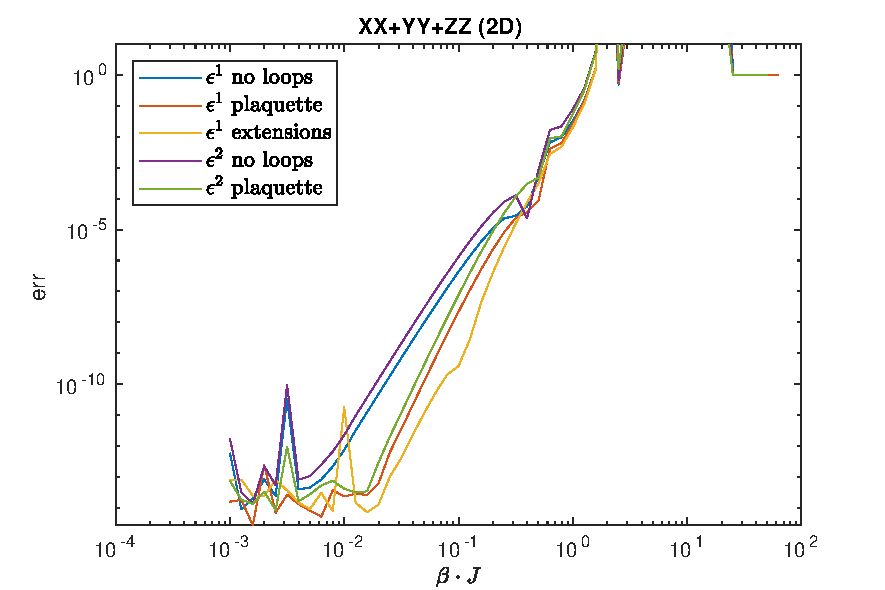
\includegraphics[width=\textwidth]{Figuren/benchmarking/2D_Err01_heis.pdf}
    \caption{The errors $\epsilon^i$ for 2D Heisenberg model. }
    \label{fig:res2d:n1:heis}
\end{figure}

\subsection{Conclusion}

It is interesting to compare the no loops errors from 2D with ( \cref{fig:benchmark:tising} A:5) and (\cref{fig:benchmark:tHeisenberg} A:5), the equivalent 1D errors.  They roughly match up, as can be expected. A similar observation can be made for lower order constructions.

This places the additional improvement of the error due to single extensions into context: they make an improvement, but one can expect the higher order expansion with same bond dimension to be just as successful.

In general, the results above show that the cluster expansions are also promising in 2D setting. The fact that the version with plaquette extensions works well also opens up the pathway for simulations in higher dimension. The computation of the 'linear' blocks scale with the number of legs. The generalisation from 2x2 plaquette term to 2x2x2 cube should still be feasible, as the solvers are cable of handling systems with 8 sites.